%-----------------------circuit 1--------------------------
\section{Single Phase Full Wave Uncontrolled Rectifier with R
  load}

\subsection{Circuit used for simulation}

% figure that is centered on the page
\begin{figure}[h]
    \centering
    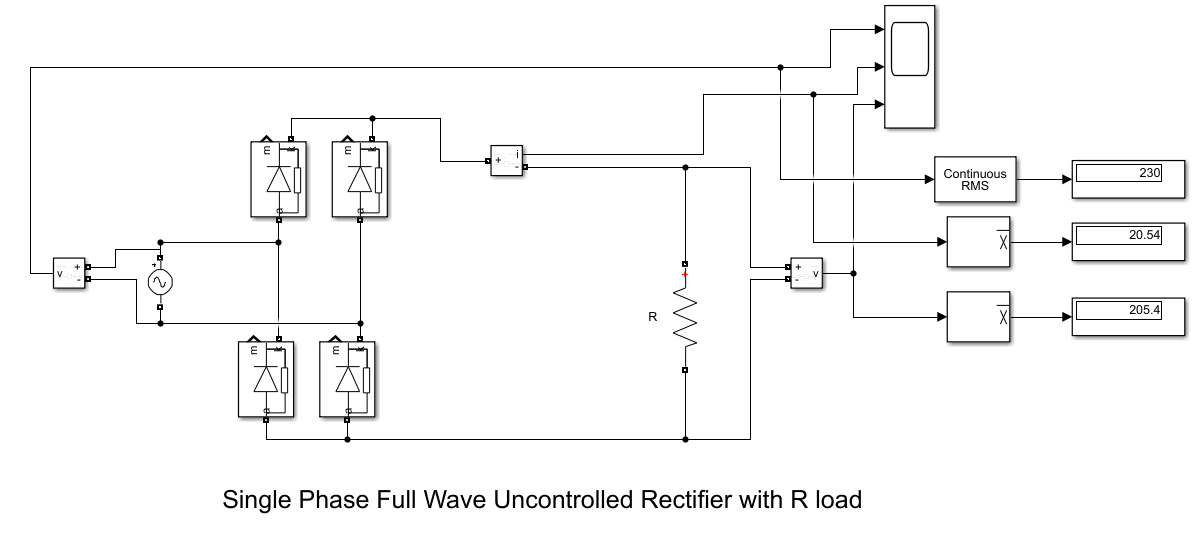
\includegraphics[width=0.7\textwidth]{images/experiment-2/circuit-diagram-simulation-01.png}
    \caption{Circuit used for simulation}
    \label{Fig_simulation_circuit_single-phase-full-wave-uncontrolled-rectifier-with-R-load}
\end{figure}

\subsection{Components Required}

\begin{table}[h]
    \renewcommand{\arraystretch}{1.3}
    \label{table_components_required_circuit_1}
    \centering
    \begin{tabular}{|c|c|c|c|}
        \hline
        Sr. No & Parameters                     & Ratings            & Quantity \\
        \hline
        \hline
        1      & AC Single Phase Voltage Source & 230V ($ V_{rms} $) & 1        \\
        \hline
        2      & Resistor                       & 10$ \Omega $       & 1        \\
        \hline
        3      & Diode                          & -                  & 1        \\
        \hline
        4      & Voltmeter                      & -                  & 2        \\
        \hline
        5      & Ammeter                        & -                  & 1        \\
        \hline
    \end{tabular}
    \caption{Components for Single Phase Full Wave Uncontrolled Rectifier with R load}

\end{table}




\subsection{Observations}

\begin{table}[h]
    \renewcommand{\arraystretch}{1.3}
    \label{table_observation_circuit_1}
    \centering
    \begin{tabular}{|c|c|c|}
        \hline
        Parameters                              & Theoretical Values & Simulation Values \\
        \hline
        \hline
        AC Input Voltage ($ V_{in,rms} $)       & 230V               & 230V              \\
        \hline
        Output Average Voltage ($ V_{o,avg} $)  & 207.07V            & 204.3V            \\
        \hline
        Output Average Current ($ I_{o,avg}  $) & 20.70A             & 20.43A            \\
        \hline
        DC Input Power ($ P_{DC}  $)            & 4218.916W          & 4173W             \\
        \hline
        Efficiency (\%)                         & 79.73              & 79.73             \\
        \hline
    \end{tabular}
    \caption{Observations for Single Phase Full Wave Uncontrolled Rectifier with R load}

\end{table}


Upon careful observation, it can be inferred that the simulated values exhibit a close resemblance to their theoretical counterparts. Given that the load is resistive, the output current waveform is found to be in phase with the output voltage waveform. Moreover, it is worth noting that as a result of full-wave rectification of the input AC signal, the output DC signal is characterized by a frequency that is double that of the input signal.
\pagebreak

\subsection{Resultant Waveforms}

% figure that is centered on the page
\begin{figure}[h]
    \centering
    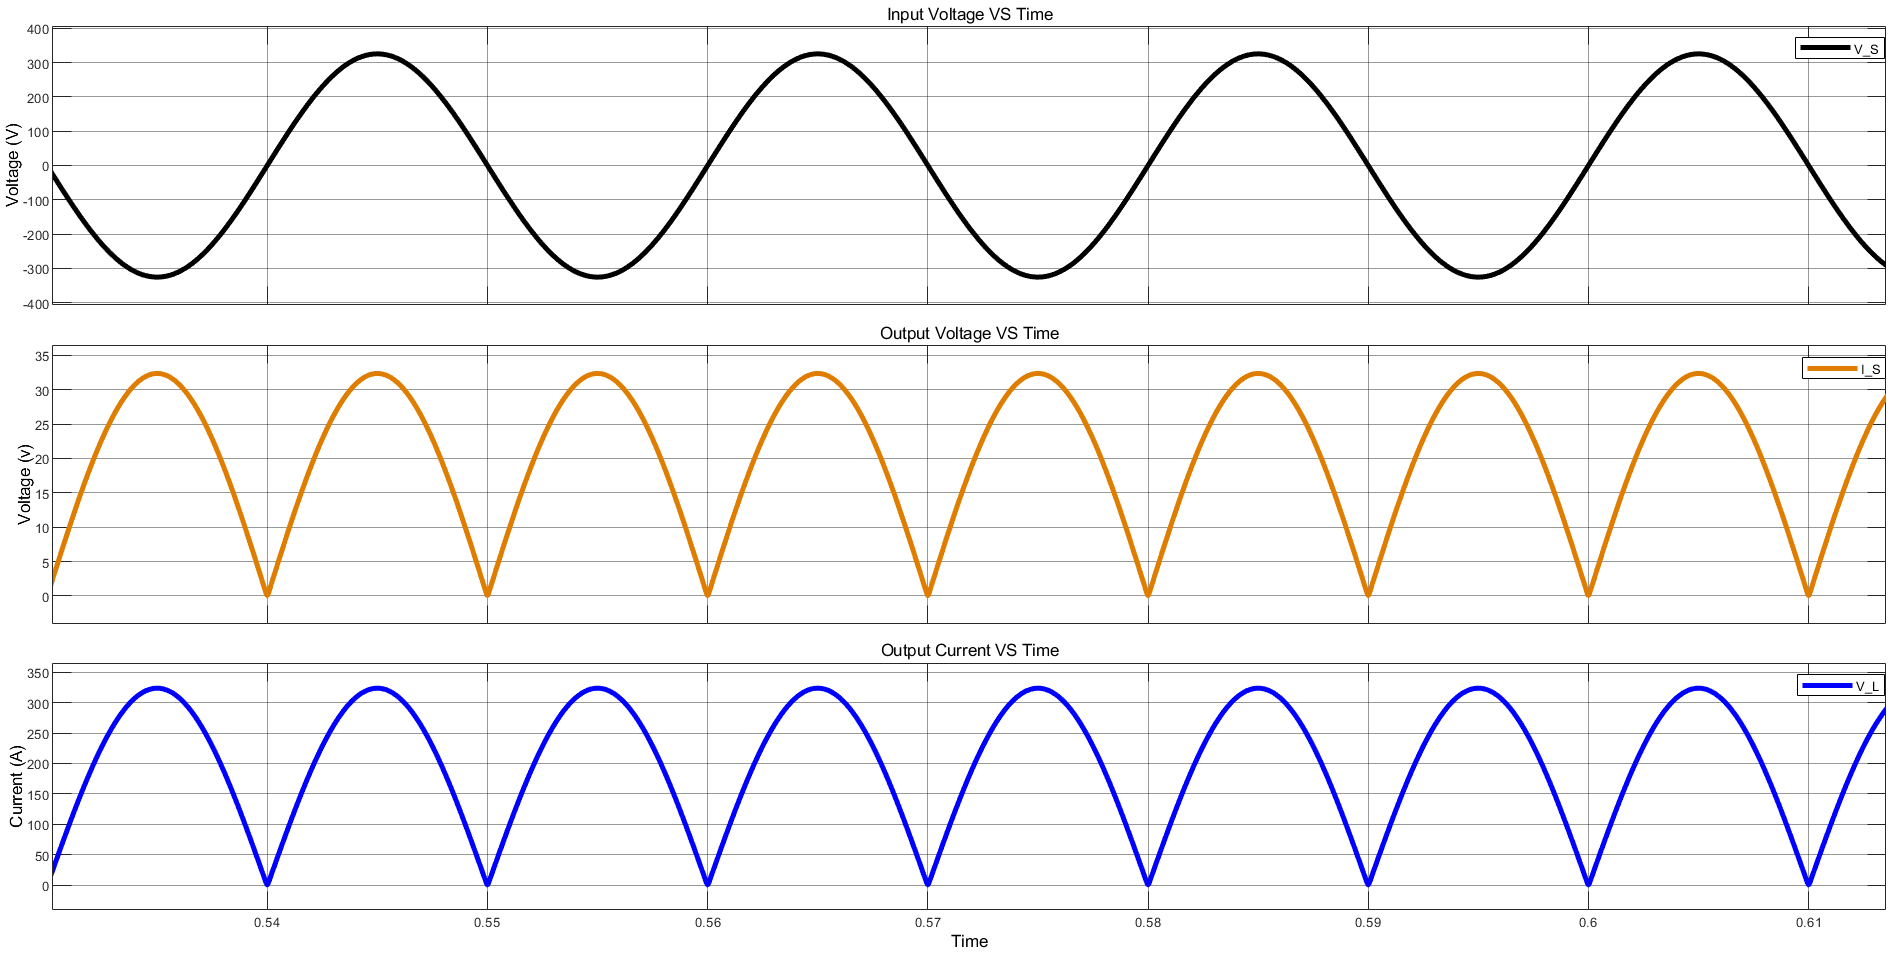
\includegraphics[width=1\textwidth]{images/experiment-2/circuit-scope-simulation-01.png}
    \caption{Scope Waveforms for Single Phase Full Wave Uncontrolled Rectifier with R load waveforms}
    \label{Fig_waveform_single-phase-full-wave-uncontrolled-rectifier-with-R-load}
\end{figure}

\pagebreak